

\section*{Einleitung}
Diese Arbeit beschäftigt sich mit der Layout-Segmentierung von Digtalisierten Dokumenten mittels Neuronaler Netzwerke.

\cref{chap:documents} beschreibt die Motivation für die Dokumentensegmetierung und aktuelle Entwicklungen im
Bereich der Dokumentendigitalisierung.

\cref{chap:theorie} beschreibt die Theorie der Künstlichen Neuronalen Netzwerke.

\cref{chap:reproduktion} setzt sich mit den mit zwei Forschungsergebnisse der Dokumentensegmetierung auseinander indem 
versucht werden zusle

\cref{chap:selfsupervised} erläuter die Methode des selbstüberwachten Lernen. Die Methode wird auf die reproduzierten Forschungen angewendet.

\cref{chap:umsetzung} erläutert Details, Probleme und Ergebnisse der umgesetzten
Reproduktionen und dem Einsatz von selbstüberwachten Lernen.

%-------------------------------------------------------------------------------
\chapter{Digitalisierte Dokumente}
\label{chap:documents}
% Warum scannt man Dokumente

% Was für Dokumente werden gescannt

% 
Schon in den 50er Jahren begann die Forschung im Bereich der Optischen Zeichenerkennung 
(engl. OCR)\autocite{DoermannHandbookdocumentimage2014}. OCR fand zuerst Einsatz in genau 
spezifizierten Problembereichen zum Beispiel die Erkennung von Druckbuchstaben einer Schreibmaschine. 
Je mehr Dokumente digitalisiert wurden, desto klarer wurde es das Dokumente mehr als 
eine Kette von Zeichen sind. 
Information können in Dokumenten über die Position der Zeichen und Skalierung von Zeichen vermittelt werden.
Zum anderen bestehen Dokumente aus Inhalten die semantische Bedeutung haben, aber nicht als Zeichenkette codiert werden können. 
Eine Randnotiz\marginnote{Der Bezug dieses Satzes zum Text wird durch die Position verdeutlicht} setzt sich durch Formatierung und Position vom restlichen Text ab. 

Wirtschaftsinteressen trieben die Entwicklungen von Dokumentenverarbeitungssystemen in einigen Bereichen sehr weit voran, wie 
zum Beipspiel bei der Verarbeitung von Geschäftsbriefen und Formularauswertung.
Eine Spezialisierung auf bestimmte Dokumentenklassen ist immer noch eine notwendigkeit angesichts der unzähligen, veränderbaren und nicht fest gelegten Gestaltungsmöglichkeiten für Dokumente \parencite[69]{BairdEvolutionDocumentImage2014}.


\section{Digitale Bibliotheken}
\cite{BairdDigitallibrariesdocument2003}

\section{Schritte in der Verarbeitung von Dokumentenbildern}
Die Dokumentensegmetierung ist ein Vorverarbeitungsschritt für weitere Schritte der Dokumentenverarbeitung.

Im Bereich der Bibliotheswissenschaften besteht ein großes Interesse an Klassifizierung von
Buchseiten zur besseren Erschließung.
\cite{McConnaugheyLabeledSegmentationPrinted2017} klassifizieren Buchseiten anhand von textbasierten Features in 4 Kategorien. 
Flow

\section{Auswahl und Beschreibung der Datensätze}
\textcite[985\psqq]{DoermannHandbookdocumentimage2014} listen 5 Aspekte die bei der Erstellung von Datensätzen zu beachten sind:
Auswahl der Daten
Datenbeschaffung
Ground Truth Definition
Ground Trouth Annotation
Speicherformat
Struktur und Organisation

\section{DIVA-HisDB}
Die DIVA \marginnote{\url{http://diuf.unifr.ch/main/diva/}}(Document, Image and Voice Analysis) Gruppe der Universität Fribourg hat im Kontext der Forschungsprojekte HisDoc und HisDoc 2.0 
das Datenset DIVA-HisDB. erstellt.
Die HisDoc-Projekte beschäftigen sich mit der automatischen Analyse von historischen Dokumenten und
wie man diese für Historiker nutzbar machen kann.

Für den Datensatz wurden Dokumente mit komplexen Layout aus der Virtuellen Manuskriptbibliothek der Schweiz (\url{http://www.e-codices.unifr.ch/en}) ausgesucht. Die Manuskripte enthalten neben dem Haupttext auch Randnotizen und Text-Dekorationen. Randnotizen befinden sich auch teilweise zwischen den Zeilen des Haupttexts.
 
DIVA-HisDB besteht aus 150 Dokumenten, aufgeteilt in Trainings-, Validierungs- und Testset (siehe \cref{table:hisdb_pages}. Hinzu kommen 30 Seiten die 
für die finale Wertung des Wettbewerbs ``ICDAR2017 Competition on Layout Analysis for Challenging Medieval Manuscripts'' verwendet wurden.

\begin{table}
    \caption{Aufteilung der Seiten des DIVA-HisDB-Datenssets}
    \label{table:hisdb_pages}
    \begin{tabular}{lccccc}
        {\bfseries Name} & {\bfseries Auflösung} & {\bfseries Training} & {\bfseries Validierung} & {\bfseries Test} & {\bfseries Test ICDAR 2017)}\\
        \csvreader[head to column names]{tables/diva_hisdb_specs.csv}{}%
        {\name&	\width \(\times\)\height & \train	&\validate	&\test	&\comp\\}
    \end{tabular}
\end{table}

Die Manuskripte wurden mit einer Auflösung von 600 dpi gescannt und sind im  JPEG-Format gespeichert. Die \cref{table:hisdbsamples} zeigt Beispiele aus den drei Datensätzen. 



Der Datensatz wurde semi-automatisch mit 3 Annotation (Haupttext, Kommentare, Dekorationen) versehen.
Diese Ground-Truth-Annotationen sind im PAGE-XML-Format und als ``pixel-label'' PNG-Bilder gespeichert.
Die Menge an Pixeln pro Klasse ist sehr unterschiedlich.
Die \cref{table:class_distribution} zeigt das in jedem Dokumentenset der Hintergrund deutlich überwiegt.

\begin{table}
    \caption{Verteilung der Klassen in Prozent\autocite[1362]{SimistiraICDAR2017CompetitionLayout2017}}
    \label{table:class_distribution}
    \begin{tabular}{lrrrr}
        {\bfseries Set} & {\bfseries Hintergrund} & {\bfseries Kommentar} & {\bfseries Dekoration} & {\bfseries Text}\\
        \csvreader[head to column names]{tables/diva_hisdb_class_distribution.csv}{}%
        {\set&	\background & \comments & \decoration & \text \\}
    \end{tabular}
\end{table}


\begin{table*}
    \begin{tabular}{llp{4cm}}
        \vspace{0.2cm}
        {\bfseries Seite} & {\bfseries Detailauschnitt} & {\bfseries Quelle } \\
        \vspace{0.5cm}
        
        \raisebox{-.5\height}{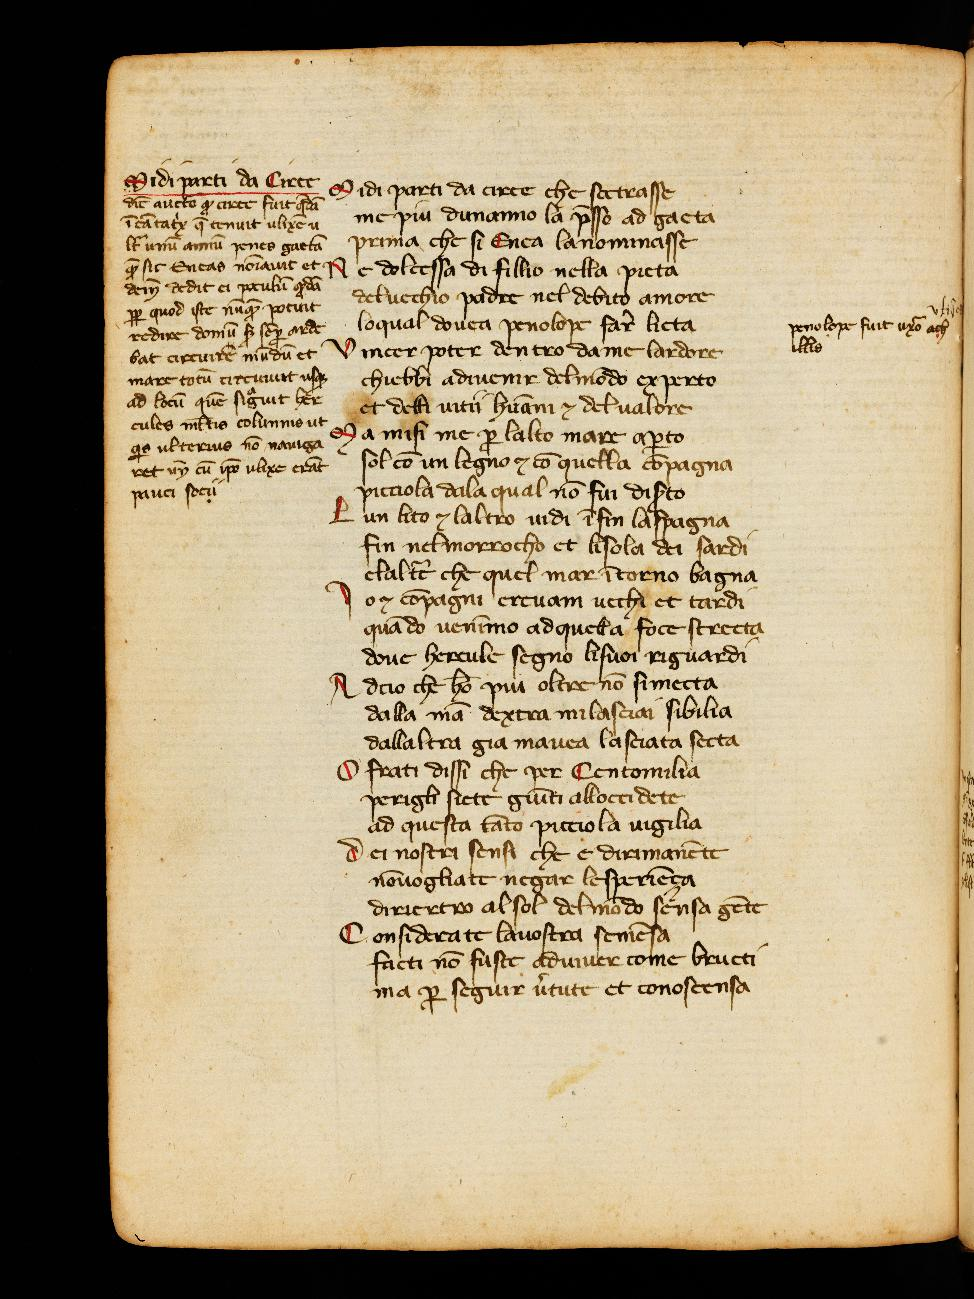
\includegraphics[height=4cm]{figures/datasets/HisDBSample0.jpeg}}
    &\raisebox{-.5\height}{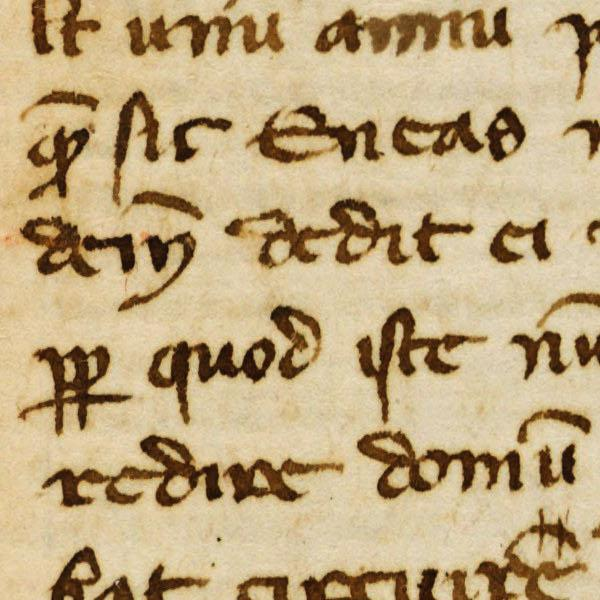
\includegraphics[height=4cm]{figures/datasets/HisDBSampleBox0.jpeg}}
     & \citefield{AlighieriColognyFondationMartin1300}{title}\\
     \vspace{0.5cm}  
     
    \raisebox{-.5\height}{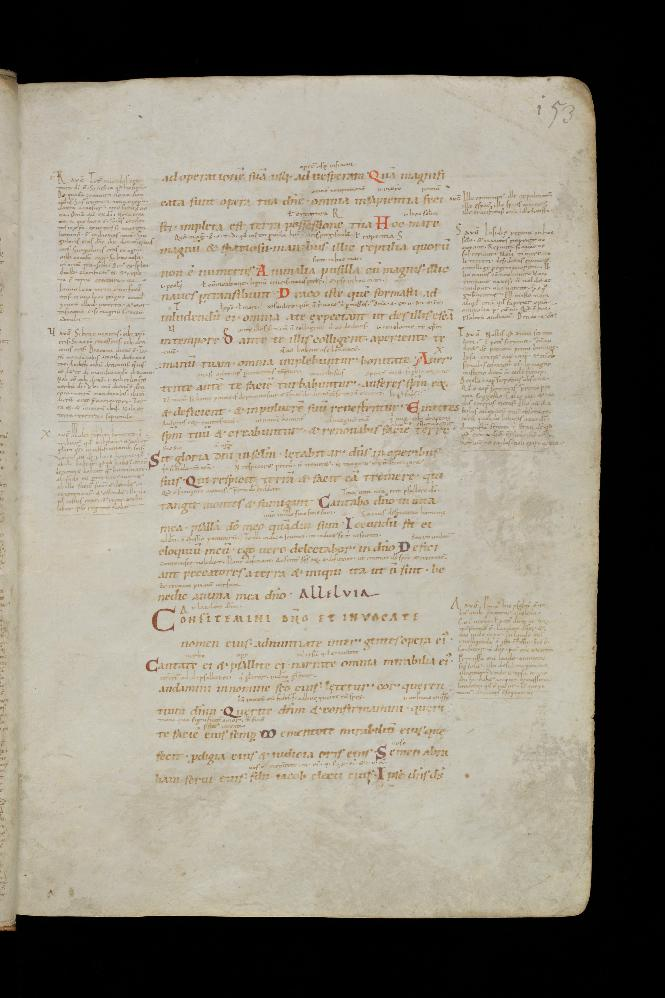
\includegraphics[height=4cm]{figures/datasets/HisDBSample2.jpeg}}
    & \raisebox{-.5\height}{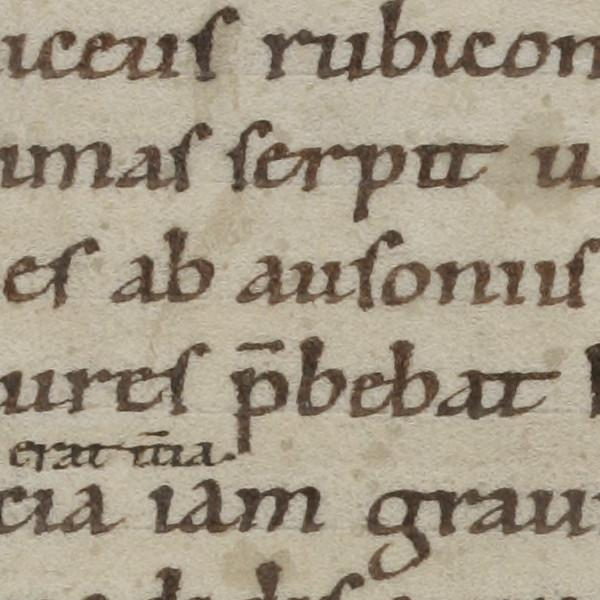
\includegraphics[height=4cm]{figures/datasets/HisDBSampleBox2.jpeg}}
    & \citefield{AmbrosiusStGallenStiftsbibliothek985}{title}\\
    \vspace{0.5cm}
    
     \raisebox{-.5\height}{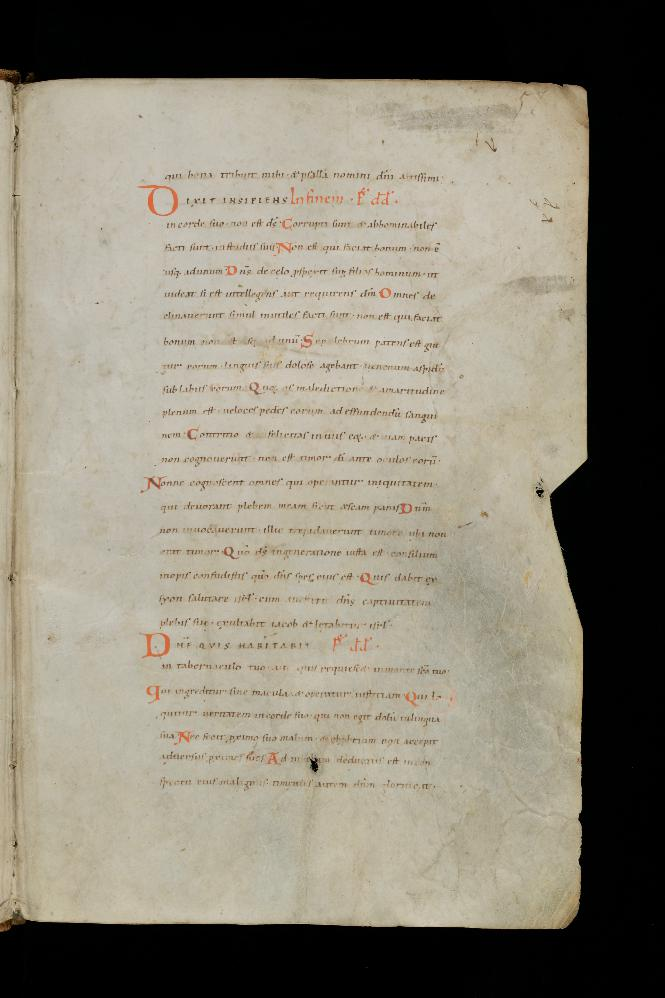
\includegraphics[height=4cm]{figures/datasets/HisDBSample1.jpeg}}
    &\raisebox{-.5\height}{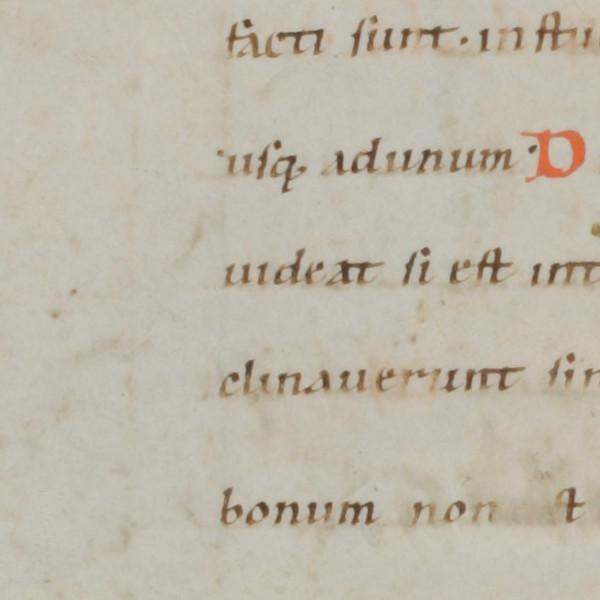
\includegraphics[height=4cm]{figures/datasets/HisDBSampleBox1.jpeg}}
     & \citefield{LucanusStGallenStiftsbibliothek1025}{title}\\
     \vspace{0.5cm} 

    \end{tabular}
    \caption{HisDB Beipsiele mit Detailauschnitt}
    \label{table:hisdbsamples}
\end{table*}


%-------------------------------------------------------------------------------
\chapter{Theoretische Grundlagen}
\qq{Warum NN?}
Künstliche Neuronale Netzwerke (kurz NN) dominieren den Forschungsbereich der 
Bilderkennung. 
Besonders die Klasse der faltenden Neuronalen Netzwerks \engl{convolutional neural network}, kurz CNN, konnte viele Erfolge für sich beanspruchen.
Rekordbrechende Ergebnisse bei der Klassifiziererung von handgeschriebenen Ziffern \parencite{LeCunBackpropagationappliedhandwritten1989} und des ImageNet-Wettbewerbs \parencite{KrizhevskyImageNetClassificationDeep2012} motivieren dazu CNN-Methoden auch in anderen
Bereichen anzuwenden.

\begin{marginfigure}
    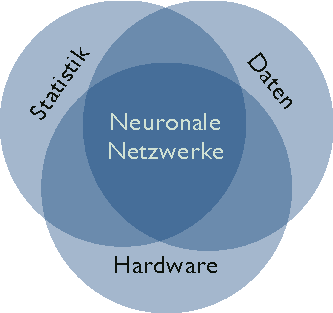
\includegraphics[width=\textwidth]{figures/tasks/nn_areas_venn.pdf}
    \caption{Diziplinen im Bereich Neurale Netzwerke}
    \label{fig:chen:cnn_task}
\end{marginfigure}
Neurale Netzwerke benötigen weniger Entwicklungsaufwand und können zudem einfacher von 
 wachsenden Rechenkapazitäten und Datenmengen gebrauch machen \parencite[436]{LeCunDeeplearning2015}. 
Aber die Wissenschaft der NN ist ein Feld, dass durch die aktuelle Praxis mehr als durch Theorie geprägt ist. 
Das bedeuted zum einen das theoretische Grundlagen noch nicht gefestigt sind.
Zum anderen ist die Theorie nur eine Faktor für den erfolgreichen Einsatz von NNs. 
Je mehr Parameter unklar sind desto schwieriger wird eine Reproduktion.
\qq{Unterschied replikation, reproduktion?}
Die Reproduktion von Ergebnissen ist aber ein wichtiger Bestandteil in jedem Forschungsgebiet. 

\section{Einführung Maschinelles Lernen}
Neurale Netwerke und CNN sind Beispiele für Machinenlernalgorithmen \engl{maschine learning algorithms}.
\cite{MitchellMachinelearning1997} definiert einen Machinenlernalgorithmus wie folgt: ``A computer program is said to learn from experience E with respect to some class of tasks T and perfomance measure P, if its performance at tasks T, as measured by P improves with experience E''.

% experience E 
Die Erfahrung E kann zum Beispiel ein Datensatz \(X\) mit zugehörigen Klassen
\(Y\) sein. Im Fall der Dokumentensegmentierung kann ein Element \(x_i\) ein Bildauschnitt sein, 
dessen Kategorisierung ist dann das Label \(y_i\)(siehe \cref{fig:chen:cnn_task}).
\begin{marginfigure}
    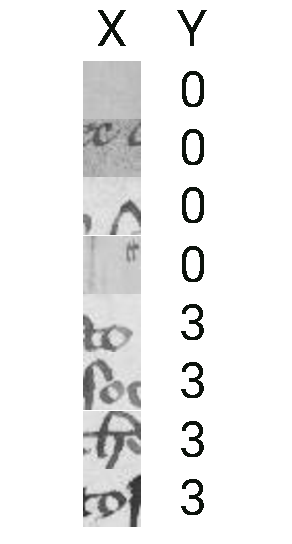
\includegraphics[width=\textwidth]{figures/tasks/chen_examples.pdf}
    \caption{Bildauschnitt mit ground ground truh (0: Hintergrund, 3: Haupttext)}
    \label{fig:chen:cnn_task}
\end{marginfigure}

% Task T 
Die Aufgabe T ist in den meisten Fällen eine statistische Modellierung.
Es wird angenommen, dass \(X\) und gegebenfalls \(Y\) mithilfe einer Wahrscheinlichkeitsfunktion \(p\)
modeliert werden können. 
Ein unüberwachter Lernalgorithmus versucht die Verteilung \(p(x)\) direkt zu lernen.
Beispiele für unüberwachte Algorithmen sind der k-Means-Algorithmus oder der PCA-Algorithmus.

Bei überwachten Lernalgorithmen wird versucht die Wahrscheinlichkeitsverteilung \(p(y | x)\) implizit zu ``lernen''.
Der Lernalgorithmus soll dabei eine Funktion finden \(f: \mathds{R}^n \rightarrow \left\{1,\dots,k \right\} \) so das \(y = f\left(x\right)\) \parencite[97 ff]{GoodfellowDeeplearning2016}.
Ein Lernalgorithmus der diese Funktion findet ist ein überwachter Lernalgorithmus \engl{supervised learning algorithm}
Die Trennung zwischen überwacht und unüberwacht ist nur eine grobe Einteilung. Tätsächlich sind die übergänge fließend. 
Manche Machinenlernverfahren benutzen beide Methoden.  

% perfrmance P
Die Performanz P der Vorhersagefunktion \(f\) wird im einfachsten Fall mit der Genauigkeit,
dem Verhähltniss von richtigen Vorhersage zu Falschen, gemessen. 
% TODO: Tabelle
\cref{tab:truth}
\begin{table}
    \caption{Wahrheitstabelle}
    \label{tab:truth}
    \begin{tabular}{llll}
                    &&\(y\)& \\
                            && Positiv       & Negativ \\
    \(\hat{y}\) & Positiv  & true positive  & false positive \\
                & Negativ & false negatve   & true negatve \\
    \end{tabular}       
\end{table}    
\section{Künstliche Neuronale Netzwerke}

Künstliche Neurale Netwerke \kurz{KNN} sind eine Modellierungsmethode des statistischen Lernens, die von der Natur inspiriert wurde. 
Das Neuron ist der Grundbaustein eines Netwerkes und verarbeitet eingehende Signale. 
Ein KNN besteht meistens aus zwei Teilen: einer linearen Funktion über die Eingabesignale und 
einer nicht-linearen Aktivierungsfunktion.

Das einfachste Beispiel ist die Klasse der vollvernetzen KNN. 
Jedes Element in einem Eingangssignalvektor \(x\) wird mit einem Parameter aus dem Gewichtsvektor \(w\) verechnet. Dazu kommt der Biaswert \(b\).

\begin{align}
    \hat { y } = w^{ \top } x + b
\end{align}



\begin{align}
    f(X)=\sum\limits_{m=1}^{M}g_{m}\left(\omega_{m}^{\top}X\right)
   \end{align}
Target als nonlineare Funktion dieser Features modelieren.  


\section{SGD}

\section{Aktivierungsfunktionen}
\begin{align}
    \operatorname{softmax}(z)_{i}=\frac{\exp\left(z_{i}\right)}{ \sum _ { j } \exp \left( z _ { j } \right) }
\end{align}
% TODO: set font size??? 
\begin{figure}
    \caption{ReLU- und Sigmoid-Funktionsplot}
    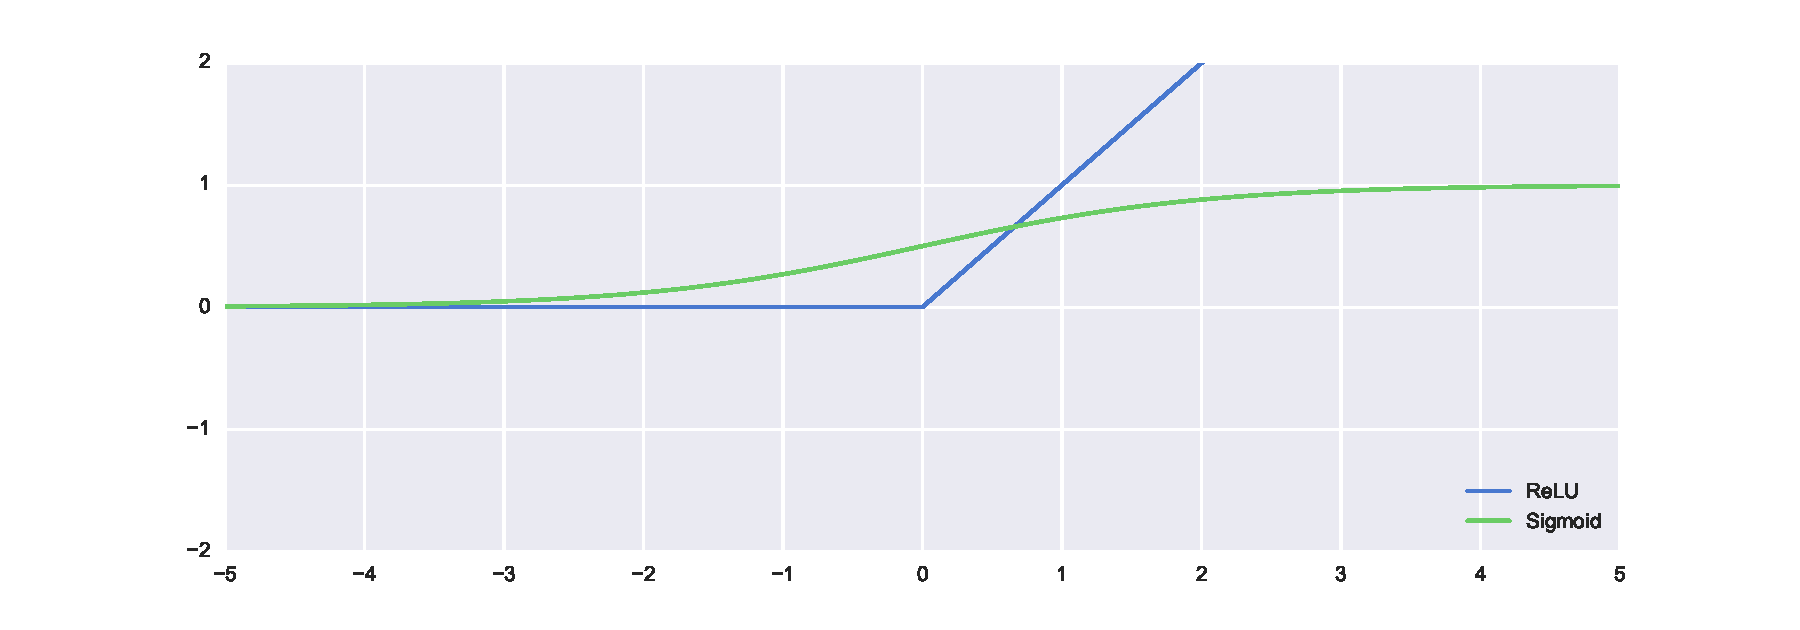
\includegraphics[width=\textwidth]{figures/plot/relu_sigmoid.pdf}
\end{figure}

\subsection{ReLU}
\begin{align}
    f\left(x\right) &= \text{max}(0,x)
\end{align}
\subsection{Softmax}


\section{Xavier initialization}

\section{Regularisierung}
\label{sec:Regularisierung}
\section{Weight decay}
\section{Dropout}



\section{CNN}
\qq{Nachtteile fully connected NN für Bilderverarbeitung}
Die Anzahl der Parameter in der Gewichtsmatrix \(W\) wird von der Größe des Inputs bestimmt.
Möchte man Bilder ein Bild mit der der 

\qq{Sind Filter vorläufer von CNN?}
CNN kombinieren zwei Konzepte der Bilderverarbeitung: Neuronale Netzwerke und Filter.
Klassifikationsprobleme wurde traditionell in zwei Schritten gelöst. Zuerst wurden 
Featuredeskriptoren entwickelt welche dann als Input für trainierbare Klassifizierer 
verwendet wurden \autocite[2353]{RawatDeepConvolutionalNeural2017}.


\qq{Was ist convolutional?}
So können zum Beipspiel Kanten in einem Bild ein Klassifizerungsgrundbaustein sein. 
Um die Kanten in einem Bild zu finden wird das Bild mit einem Kernel  gefaltet.  
Der Begriff Faltung wird üblicherweise für die Verknüpfung von zwei realwertigen Funktione verwendet. Die analoge Form der Faltung ist eine lineare , translations-invariante Funktion, siehe \cite[28]{SusseBildverarbeitungundObjekterkennung2014}. 
\begin{align}
    \label{eq:convolutional}
    convolutional
\end{align}
Im Bereich der Bilderverarbeitung wird schon länger eine abgeänderte Faltungsfunktion genutzt: die Autokorrelation \engl{cross-correlation}. Bild und Filter sind 2D-Funktionen die zum einen nur für diskrete Intervale definiert sind zum anderen für Bereiche aushalb des ihres Definitionsbereichs gleich 0 sind. Zudem wird überlicherweise der Index für den Kernel addiert (siehe \cref{eq:convolutional}).
\begin{align}
    \label{eq:crosscorrelation}
    I*K(i,j) =
\end{align}


Ein CNN ist eine Neurales Netzwerk, dass in mindesten einen Layer die Faltung anstatt der normalen Matrixmultiplikation verwendet \parencite[321]{GoodfellowDeeplearning2016}.
\qq{Drei Hauptvorteile?}
\cite{GoodfellowDeeplearning2016} sieht drei Vorteile von CNN gegenüber voll-vernetzten NN: verringerte Konnektivität, 
gemeinsame Parameternutzung, eqivariante Darstellung.
Wie schon erwahnt steigt die Anzahl der Parameter in einem voll-vernetzten NN je größer der Input wird, weil jedes Neuron mit jeder Aktivierung der vorhergehenden Schicht verbunden ist. 
Durch die Faltungssoperation erhählt jedes Neuron nur die Signale die im Bereich des Filterkernels liegen. Dieser Bereich wird auch rezeptives Feld genannnt.
Durch die Schichtung von mehreren Faltungen vergrößert sich das rezeptive Feld der Neuronen in tieferen Schichten (siehe \cref{fig:cnn_neurons}).


\begin{marginfigure}
    \label{fig:cnn_neurons}
    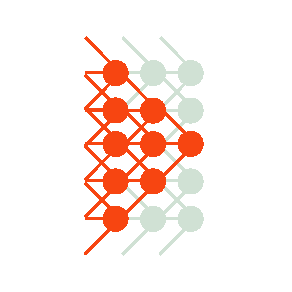
\includegraphics[width=\textwidth]{figures/sketch/cnn/perceptive_field.pdf}
    \caption{Rezeptives Feld in einem mehrschichtigen Netz}
\end{marginfigure}

\qq{Nachteile CNN?}
\qq{Filterbeispiel?}
\qq{}


\section{Vorverarbeitung}

\section{SLIC Superpixel}
Der SLIC-Algorithmus basiert auf dem k-Means-Algorithmus und teilt Pixel inhalb eines 5D-Raums in Cluster ein. 
In jedem Arbeitsschritt werden Pixel dem Clusterzentrum mit der geringsten Distanz zugeordnet und danach werden die Clusterzentren neu berechnet.
Das Distanzmaß \(D_s\) zu den Clusterzentren \(k=[1,K]\) basiert auf den Farbabstand im Lab-Farbraum \(d_{lab}\) und den räumlichen Abstand \(d_{xy}\):

\begin{align}
    d_{lab} &= \sqrt{ \left( l_k - l_i \right)^2 + \left( a_k - a_i \right)^2 + \left( b_k - b_i \right)^2 }\\
    d_{xy}  &= \sqrt{ \left( x_k - x_i \right)^2 + \left(y_k - y_i \right)^2 }\\
    D_{s}   &= d_{lab} + \frac{m}{S} d_{xy}
\end{align}

Der Faktor \(m\) ermöglicht eine Gewichtung den zwei Distanzmaßen. Je höher
der Faktor desto kompakter werden die Superpixel. \cref{fig:slic_parameters}
zeigt das Ergebniss des Algorithmus mit unterschiedlichen Parameter  \(m\)
angewendet auf eine Dokumentenseite.

%-------------------------------------------------------------------------------
\import{chapters/}{reproduktion}
%-------------------------------------------------------------------------------
\import{chapters/}{selfsupervised}
%-------------------------------------------------------------------------------
\chapter{Umsetzung}
\qq{Nebenziel bei der Umsetzung}
Ziel der Arbeit war es nicht nur Ergebnisse zu reproduzieren, sondern auch selbst reproduzierbar zu sein. 
Dafür sollten alle Prozesse, Datenverarbeitungsschritte und gewählte Paramter in einheitlicher Form definiert sein.  
\subsection{Python und PyTorch}
Python ist eine objektorientierte, interpretierte Programmiersprache.
Zur Bildverarbeitung wurde die Python-Bibliothek scikitimage verwendet.
Die neuronalen Netze wurden mithilfe von PyTorch umgesetzt.
% Genauer klären
PyTorch ist ein Framework zur automatischen Differenzierung von skalarer Funktion \autocite{PaszkeAutomaticdifferentiationPyTorch2017}.
\label{chap:umsetzung}
\section{Chen}
\citeauthor{ChenConvolutionalNeuralNetworks2017a} nennen nicht die genaue Zahl des Verwendeten Kompaktheitsparameter m (siehe \cref{sec:slic}). 
Die Konfiguration der Superpixel setzt aber eine Obergrenze für die maximal erreichbare Genauigkeit.
Um den besten Paramter zu finden wurde die Bilder mit der Vorbearbeitungsmethode von \citeauthor{ChenConvolutionalNeuralNetworks2017a} in Superpixel aufgeteilt. 
Die Klassifizierung der Pixel wurde direkt aus der ground truth übernommen.
Dieser Vorgang wurde für 10 zufällige Bilder des DIVA-Datensatzes wiederholt und ein Durchschnitt gebildet.

\sfigure{Maximale Genauhigkeit in Abhängigkeit von m}{figures/datasets/slic_hyperparameter.pdf}



aslic?
Netz Lernt, aber nur MNIST
\sfigure{Fehlerrate CheNet(4,4,0) während der Trainingsiterationen}{figures/plot/run_ChenNet_MNIST_log_ChenNet4_4_01522892733-tag-training_error.pdf}
Boundary pixel werden als GT label verwendet

\section{Xu}
multilabel vorhersage?

\section{Discrimitve}

\section{Evaluierung}
\label{chap:eval}


\sfigure{Beispiel aus dem DIBCO2013-Dateset}{figures/tasks/DIBCO2013-dataset.pdf}


\subsection{Metriken}
Die Evaluierung der Ergebnisse der Segmentierung erfolgt auf Pixelebene.
\cite{LongFullyconvolutionalnetworks2015} berechnet 4 Metriken.
Sei \(n_{ij}\) die Anzahl der Pixel der Klasse \(i\) die der Klasse \(j\) zugeordnet wurden.


\newcommand{\resulttable}[3]{
    \begin{tabular}{l|r|r|r|r|r}%
    \hline
        \csvreader[head to column names, filter equal={\dataset}{#2}]{#1}{}%
        {#3}
        \end{tabular}
}
\begin{table*}
    \resulttable{results/document_image_segmentation_results.csv}{CB55}{ \name & \pixelacc & \FgPA & \meanacc & \meanIU & \fwIU\\}
    \resulttable{results/document_image_segmentation_results.csv}{CSG18}{  \pixelacc & \FgPA & \meanacc & \meanIU & \fwIU\\}
    \resulttable{results/document_image_segmentation_results.csv}{CSG863}{  \pixelacc & \FgPA & \meanacc & \meanIU & \fwIU\\}
        
\end{table*}

\section{Fazit}


